

\begin{figure}
\centerline{
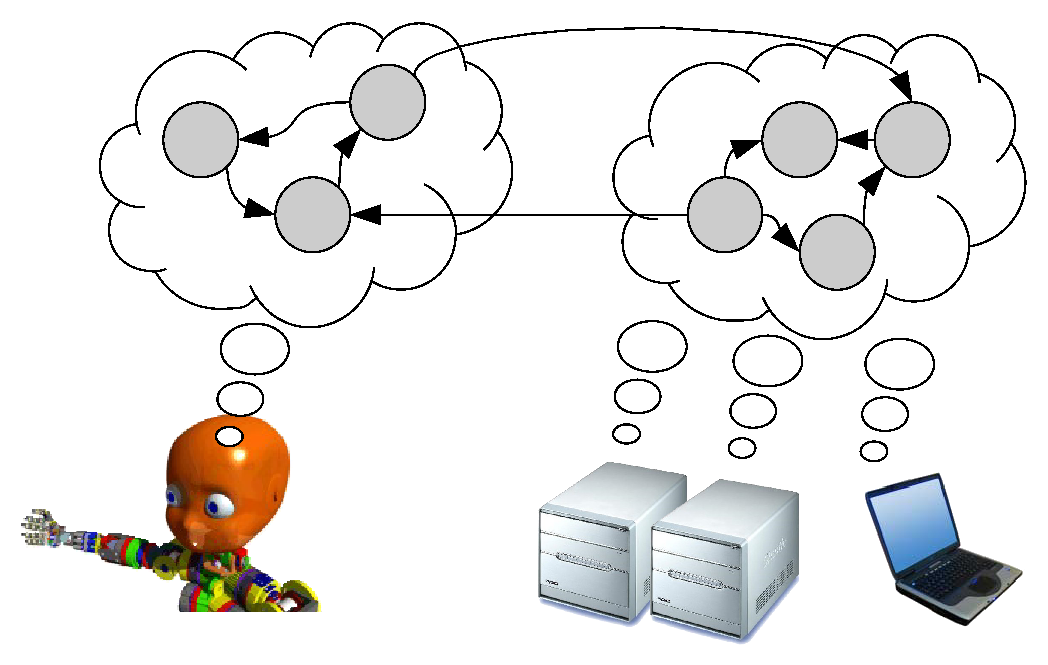
\includegraphics[width=8cm]{fig-nethead}
}
\caption{
%
Basic robot model.  We assume a set of processors, some of which may be
on the robot, some of which may not be.  We assume that the computers
are diverse: they may have different devices, operating systems,
processors, and the programs they run may use different languages,
libraries, etc.  
%
We develop methods for interfacing with devices and communicating
between modules that are useful on any heterogeneous system.
%
We extend our reach by exploiting key Free Software projects
dealing with and enabling diversity in operating systems, build systems, 
and programming languages.
%
Our contribution, made as Free Software, is a system for dealing
with and enabling diversity in transport mechanisms and novel devices.
%
%We nevertheless require that threads within processes
%on any of these computers be able to communicate easily with each other.
%
%This communication, ideally, should fit well with basic UNIX 
%tools and concepts (although we do not assume the operating systems
%in use are UNIX-based).
%
We use this software to support our open robot platform, the iCub
humanoid, whose design will be available under free and open
licensing.
%
}
\end{figure}


\section{Introduction}

%%Hardware defines the environment within which software operates.  

Robots can be very unusual software platforms to develop on, perhaps
with novel devices or uncommon processors, frequently assembled by a
team stronger in mechanical design than computer science.  In fields
such as mobile robotics some standardization can be seen, but in
humanoids idiosyncracy is the rule.  Can we avoid being a backwater for
software development?  We draw lessons from the free software community
and UNIX.


Software development is, in some ways, like natural 
evolution.  Every piece of software has its niche:
the environmental conditions within which it can be
used.  Within this niche it will grow and change and 
perhaps expand to nearby niches.
%%
Some niches are very large (for example, commercial PCs), some are
tiny (a newly developed humanoid).  In this paper, we are concerned
about how robotics researchers can avoid being caught in a tiny
niche, and how to prevent ``genetic isolation'' from setting in,
where software development is slow and cut-off from the mainstream.
We want to find a way to avoid this trap, without sacrificing
the freedom to radically change our hardware, a freedom that
will be crucial in ``bleeding-edge'' research for years to come.

Our motivation comes from the condition of humanoid robotics 
research, but most of this paper is not specific to that field.
%
We think it is relevant to any small research group, either academic or
industrial, who wishes to develop novel robots (as opposed to 
build applications on existing robots).  We want to maximize the 
reach of such research groups.


%Robots with unusual hardware can find themselves initially bereft of
%software, until adaptation occurs.  Therefore robots that take
%advantage of novel hardware may require significant software effort.


%Any given piece of software can operate in a certain set of 
%environments.  Every new robot is a new environment, with some
%overlap with existing ones.  Some software will run there,
%some will not.

%In terms of software, robotic platforms can be quite ``genetically
%isolated'' from the mainstream population of PCs.  


%Humanoid robotics is our passion, but in the grand scheme
%of world-wide software development 


%Big companies built on OSS (e.g. Google)

Robots need an analogue of the operating system of a computer, or the
nervous system of an animal.  We focus on the key issue of how information
travels between processors, sensors, and actuators.




\subsection*{Devices}

New devices come out all the time -- needs to be easy to connect them
to existing code.  YARP needs a minimal ``wrapper'' class to match
vendor-supplied library with relevant interfaces that capture common
capabilities.  YARP encourages separating configuration from source
code -- separating the ``plumbing''.  Devices and communications
remain distinct concerns.  The goal is to allow collaboration between
groups whose robots have different devices and make device changes
less painful.  We also want to have the ability to be able to switch
from remote use of device to local use and vice versa without pain,
without compromising the efficiency of local access.

